\chapter{Implementation Broker}
\label{chap:broker}


\section{Threading}
Regarding threading we mainly focus on the network layer. To support multiple
connections from different clients the acceptor socket forks a new thread for
processing incoming data whenever a new connection is established. We realized
that we need to process incoming data as fast as possible because if the limit
of the socket buffer is reached, the throughput on the network drops
dramatically. Therefore the processor threads only receive a
particular request (based on the first 4 bytes which determines request size)
and forward it to the request handler thread. Thereby, the request handler is a worker
thread which just works off the received request and produces appropriate
responses. Responses are sent to a pool of responder threads where one of them simply send the
response back to the connected client.
...

TODO: Possibility to defined a pool of request handler worker threads.
Probably we implement it, if not we have to give a statement. 

TODO: Responder pool not implemented yet (only one responder at the moment)

\begin{figure}[H]
    \centering
    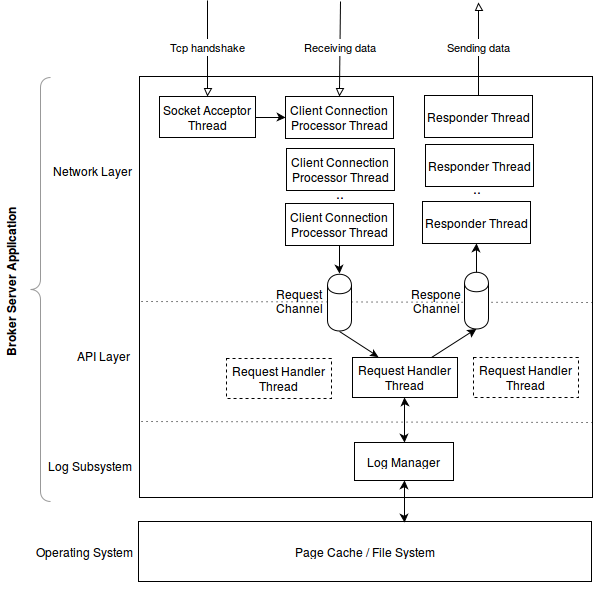
\includegraphics[width=0.7\textwidth]{images/design-threading.png}
    \caption{Threading concept which channeling}
    \label{fig:architecture-threading.png}
\end{figure}

\subsection{Channeling}

For transfering data between the threads of the subsystem API and Network, we
decided to use channels. The
\fnurl{Control.Concurrent.Chan}{http://hackage.haskell.org/package/base-4.8.0.0/docs/Control-Concurrent-Chan.html}
package provides a one-way FIFO communication channel. In
our case, this concept is being used to separate the
three mentioned subsystems from each other. The fact that
\textit{chan} is unbounded brings a risk. While
\textit{writeChan} -- which is being used to write to a
channel -- succeeds immediately, there is a chance that the
consuming thread is not able to read the same amount of
data in a given time and thus the channel will grow in
an unchecked manner. \cite{o2008real}

TODO: sanctions? do we have to block the producer for a short time?

TODO: tell why 2 separate channels are better than 1 two-way

TODO: Request Channel (ReqChan)

TODO: Response Channel (ResChan)

\section{Error Handling}

\begin{figure}[H]
    \centering
    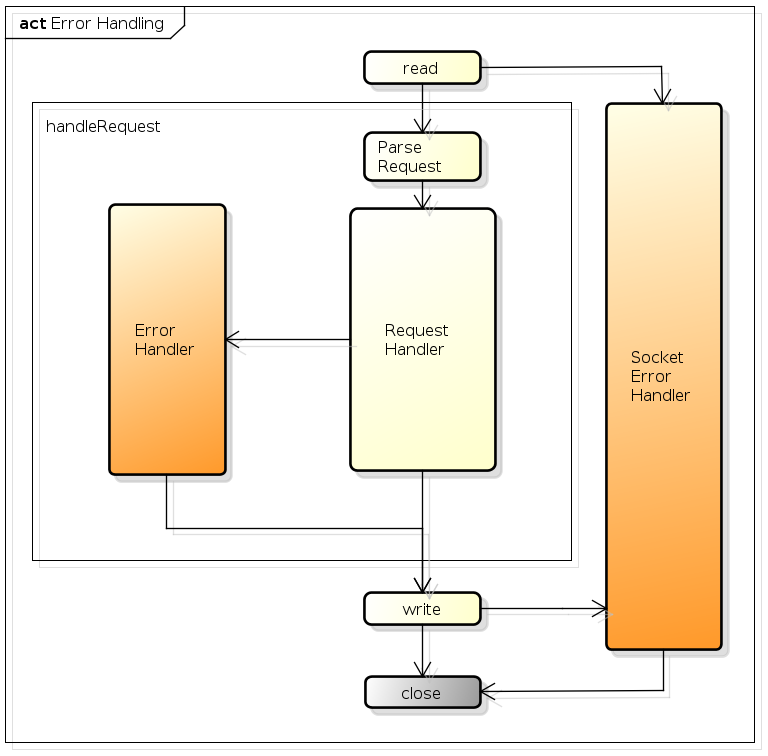
\includegraphics[width=0.7\textwidth]{images/broker-error-activity.png}
    \caption{Broker error handling concept}
    \label{fig:broker-error-activity.png}
\end{figure}


\begin{figure}[H]
    \centering
    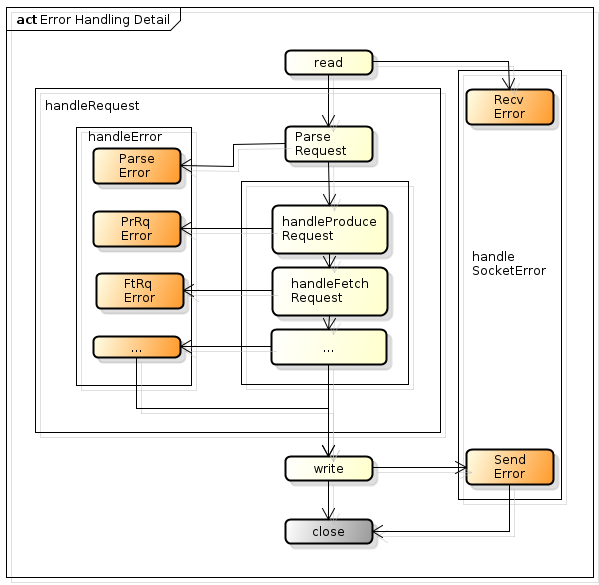
\includegraphics[width=0.7\textwidth]{images/broker-error-activity-detail.png}
    \caption{Broker handling concept in detail}
    \label{fig:broker-error-activity-detail.png}
\end{figure}

TODO: Either, Control.Monad.Error, Custom error types


\section{Network Layer}

%One of the most fundamental parts of a message broker are sockets. While a
socket is an endpoint of a bidirectional inter-process communication flow, each
connection established to the broker is basically a socket connection. That
being said, it is important to provide a reliable socket server implementation
which will serve correctly under a heavy load. Haskell provides full control
over sockets using the
\fnurl{Network.Socket}{https://hackage.haskell.org/package/network-2.3.0.7/docs/Network-Socket.html}
module which exposes the \fnurl{C socket
API}{http://pubs.opengroup.org/onlinepubs/7908799/xns/syssocket.h.html}.

\subsection{Socket connection establishment}

The following figure (\ref{fig:broker-activity}) shows the abstract view of how
the socket connection between a client and the broker establishes so that a
communication between those two counterparts can proceed.

\begin{figure}[H]
    \centering
    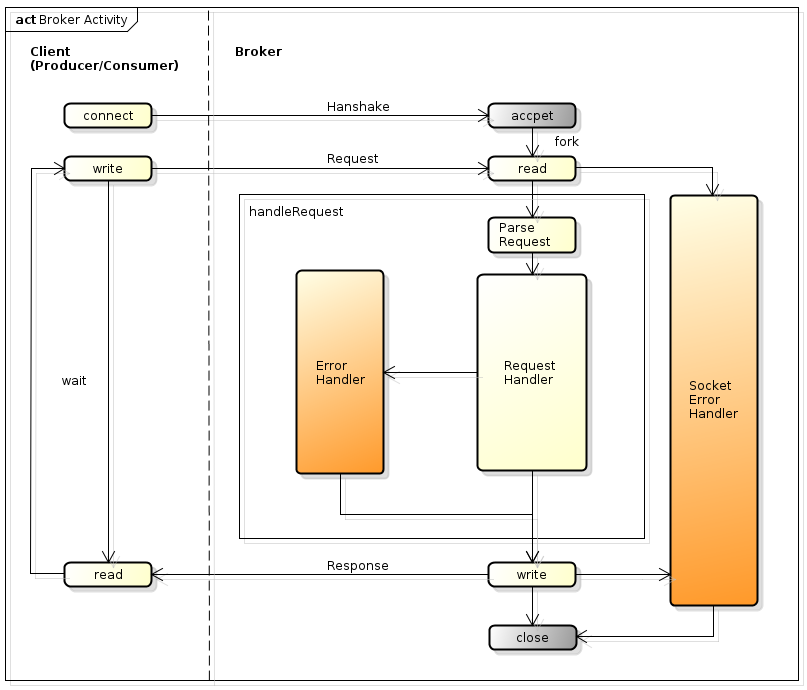
\includegraphics[width=0.7\textwidth]{images/broker-activity.png}
    \caption{Broker request handling concept}
    \label{fig:broker-activity}
\end{figure}

\subsubsection{Create Socket}

First of all, the initialization process of a socket happens on the server by providing the following configuration parameters:
\begin{description}
  \item[Protocol Familiy] \textit{AF\_INET}, for network protocol IPv4
  \item[Socket Type] \textit{Stream}, which provides sequenced, reliable, two-way, connection-based byte streams.
  \item[Protocol Number] \textit{0}, which indicates that the caller does not want to specify the protocol and will leave it up to the service provider.
\end{description}

\subsubsection{Bind Socket}

After the configuration is set, the socket has to be associated with an address
structure which is a constellation of an IP Address and Port. The constructor
\textit{SockAddrInet} of the data type \textit{SockAddr} takes the following
two arguments:

\begin{description}
  \item[Port Number] 4343
  \item[Host Address] iNADDR\_ANY, which binds the socket to all interfaces
\end{description}

TODO: static but could be done with dynamic configuration

\subsubsection{Listen}

While the socket is created and bound to an interface, the socket state can be
entered into listening state. The only configuration parameter which has to be
considered is the maximum number of queued connections they are requesting to
be accepted -- also called backlog. While this parameter is not critical in the
constellation of this broker, we set the queue length to \textbf{50}, which is
also the default value in the Java SocketServer implementation. \textit{Note,
that the focus remains on the amount of data being processed rather than the
number of clients being served.}

\subsection{Receive data}
To receive data from socket buffer we use the function recv from
\fnurl{Network.Socket.ByteString.Lazy}{https://hackage.haskell.org/package/network-2.3.0.1/docs/Network-Socket-ByteString-Lazy.html}
library which provides access to the unix socket interface. Because we work
with a binary protocol and need to parse the data from binary data directly,
this module is much more efficient than the string based network functions. We
take the lazy variant of the library because the input gets directly parsed by
our lazy based encoder \todo{ref}.

Because we want to handle each request individually we explicitly read
only the exact amount of bytes which is needed get one particular request from
the socket buffer. To get the size of a whole request we read the first four
bytes which determines the request size according to the protocol and parse it
to an numeral value.

\begin{lstlisting}
import qualified Network.Socket.ByteString.Lazy as S 
import qualified Data.ByteString.Lazy as BL

recvFromSock :: (Socket, SockAddr) -> IO BL.ByteString
recvFromSock (sock, sockaddr) =  do 
    respLen <- S.recv sock (4 :: Int64
    let parsedLen = getLength respLen
    req <- recvExactly sock parsedLength 
    where
        getLength = runGet $ fromIntegral <$> getWord32be
\end{lstlisting}

After getting the size of a particular request, this determined amount of bytes
is received from socket. Because of the blocking semantics of unix sockets and
tcp packet fragmentation it is not guaranteed, that the len argument to the recv
system call gets the exactly number of bytes of the whole request. The call may produce
less data than specified. Therefore we implement the following function to get
the data in
chunks until the entire request is read. 

\begin{lstlisting}
recvExactly :: Socket -> Int64 -> IO BL.ByteString 
recvExactly sock size = BL.concat . reverse <$> loop [] 0 
  where
    loop chunks bytesRead
        | bytesRead >= size = return chunks
        | otherwise = do  
            chunk <- S.recv sock (size - bytesRead)
            if BL.null chunk 
              then return chunks 
              else loop (chunk:chunks) $! bytesRead + BL.length chunk 
\end{lstlisting}

\subsection{Send data}


\section{API Layer}

\begin{figure}[H]
    \centering
    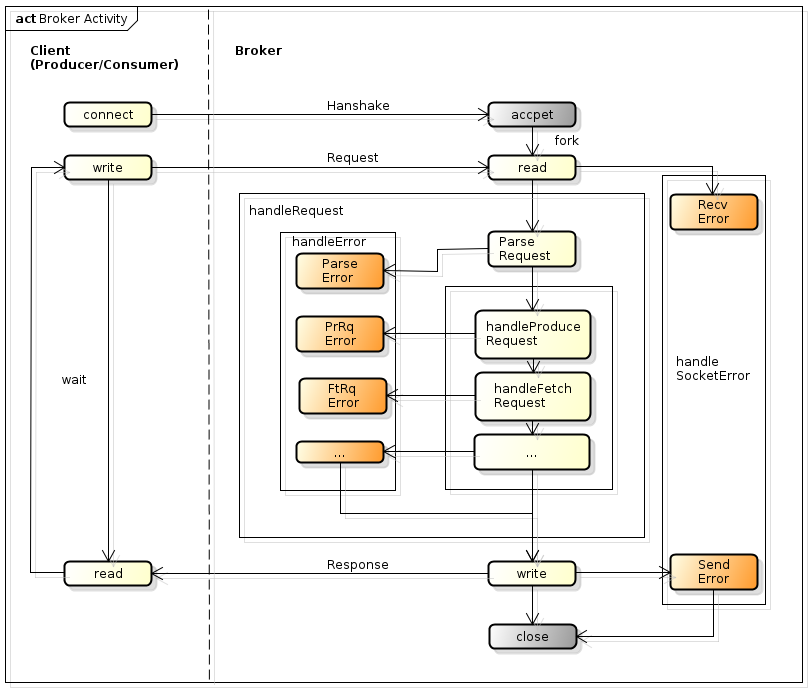
\includegraphics[width=0.7\textwidth]{images/broker-activity-detail.png}
    \caption{Broker request handling concept in detail}
    \label{fig:broker-activity-detail.png}
\end{figure}


\section{Log}

\subsection{Indexing}

\subsection{Storage Layout}
\label{broker-storage}

\subsubsection{Folder structure}

The storage layout is exactly the same as the one defined for for Apache Kafka.
\todo{link} As for now, the root location of the log is not configurable and
set to the folder named \textbf{./log} within the installation directory of the
broker. Each folder represents a partition of a specific topic whereas the name
of the folder is a combination of the topic name and the partition number. 

For example the topic named \textit{myTopic} with the partitions \textit{0} and
\textit{1} will result in the following folder structure:

\begin{itemize}
    \item ./log/myTopic\_0
    \item ./log/myTopic\_1
\end{itemize}

\subsubsection{Files}

There are two types of files they reside within the folder that specifies the
topic and partition (see folder structure):

\begin{description}
    \item[.index] Containing a sequence of index entries
    \item[.log] Containing a sequence of log entries
\end{description}

Both of the file types hold the same name which stays for the base offset and
can be considered as an unique identifier representing a 64 bit integer as a 20
character file name. As it was defined for Apache Kafka, the base offset is the
offset of the first log entry. For example if a log holds messages whereas the
first message has the offset \textit{5 :: Int64} the file name of this log will
be \textit{00000000000000000005.log} and the related index file
\textit{00000000000000000005.index}.

Using this naming convention and by
viewing multiple log files one can extract information about what range of
messages reside in which log. This is a very efficient way to perform a lookup
which is needed for example to append new log messages or archive old messages.

\subsubsection{Index on-disk format}

An index entry consists of the following two fields whereas both of them are 4 bytes each:

\begin{description}
    \item[Relative offset] 4 Bytes offset relative to the base offset (file name)
    \item[Physical position] 4 Bytes physical offset relative to the beginning of the log file
\end{description}

The relative offset of an index entry added with it's base offset represents an
actual message within the log. The second information, the physical position then tells on what 
position the message resides within the log. Thus, log access of O(n) becomes possible.

\subsubsection{Log on-disk format}

The log contains a sequence of log entries whereas the on-disk format of a log
entry is is part of the reason why the Apache Kafka becomes that valuable. In
fact, the on-disk format is exactly the same as the format of the MessageSet
(see \ref{impl-protocol-types-data}) transmitted with a ProduceRequest
\todo{add requests to protocol and link this}. Thus, data does not have to be
modified in any way and can directly be extracted and written to the file
system.

\todo{move the below to protocol}
- log entry: N (4 byte integer -> message length) followed by message (N message bytes)
- message: unique identifier (64 bit integer offset -> byte position of the start of this message in the stream of all messages ever sent to that topic on that partition)

On-disk format of a message:

offset: 8 bytes
message length : 4 bytes (value: 1+4+n) 
magic value  : 1 byte
crc            : 4 bytes
payload        : n bytes
    ?:              : 1 byte
    ?:              : 4 bytes
    message length  : 4 bytes
    message         : n bytes

\subsection{Types}

\begin{table}[H]
\resizebox{\textwidth}{!}{%
\begin{tabular}{|l|l|l|}
\hline
\textbf{Type synonym} & \textbf{Parameter}           & \textbf{Description}                     \\ \hline
TopicStr              & String                       & Parsed topic name as String              \\ \hline
PartitionNr           & Int                          & Parsed partition number as Int           \\ \hline
FilemessageSet        & {[}MessageSet{]}             &                                          \\ \hline
OffsetIndex           & {[}OffsetPosition{]}         &                                          \\ \hline
LogSegment            & (Log, OffsetIndex)           &                                          \\ \hline
RelativeOffset        & Word32                       & 4 Byte offset relative to the BaseOffset \\ \hline
FileOffset            & Word32                       & 4 Byte physical offset of a Log file     \\ \hline
OffsetPosition        & (RelativeOffset, FileOffset) & Tuple of relative and physical offset    \\ \hline
BaseOffset            & Int                          & 8 Byte offset as Int                     \\ \hline
\end{tabular}
}
\end{table}

\subsection{Write a log}

Writing data, type of MessageSet \todo{ref to type}, to a log is the
fundamental process behind the scenes of handling a ProduceRequest \todo{ref
to request}. But before actually writing data to the file system, several
steps come in between and will contribute significantly to the concept of
Apache Kafka's Log system \todo{ref to kafka log}. This section describes
the implementation details of the mentioned steps in the order of occurrence.

\subsubsection{Base Offset}

The incoming request -- which is at this point already parsed -- contains the
topic as well as the partition number for the given set of messages. Thus, we
can identify the location of the related log file. Given the location only, we yet do
not know which file we actually have to.
The file we want to write to is the one named after the highest offset,
which is why we do not get around reading the content of this directory. While doing so,
string transformations have to be applied to identify the correct offset and thus the
file to write to. Handling the case where no file exists leads
to the creation of a new log with the offset of zero.
\\

Before applying filters and string transformations, the list of files has to be
build. The library
\fnurl{System.Directory}{http://hackage.haskell.org/package/directory-1.2.2.1/docs/System-Directory.html}
provides the function \textit{getDirectoryContents} that takes a file path as a
string and returns a list of all entires in the directory. This operation
performs I/O and thus the return type is an IO monadic value. \textit{As
described on
\fnurl{hackage}{http://hackage.haskell.org/package/directory-1.2.2.1/docs/System-Directory.html\#v:getDirectoryContents},
there are several causes why this operation may fail but at this point, we do
not provide proper error handling.}

Now Haskell can perform it's beauty. To get the list of all offsets within
the directory, the function \textit{offsetFromFileName} extracts the offset
as an \textit{Int} from a \textit{String}. As an example,
\textit{"00000000000000000005.log" :: String } will be transformed to
\textit{0000000000000000005 :: Int}:

\begin{lstlisting}
offsetFromFileName :: [Char] -> Int
offsetFromFileName = read . reverse . snd . splitAt 4 . reverse
\end{lstlisting}

The function \textit{offsetFromFileName} can be mapped over a filtered list of
strings, which will give the list of all offsets within the directory. The
filter function basically omits the files other than the ones ending with
\textit{".log"} as well as the root directories, typically \textit{".", ".."}.


\begin{lstlisting}
getBaseOffsets :: (TopicStr, Int) -> IO [BaseOffset]
getBaseOffsets (t, p) = do
dirs <- getDirectoryContents $ getLogFolder (t, p)
return $ map (offsetFromFileName) (filter (isLogFile) (filterRootDir dirs))
\end{lstlisting}

Finally, the highest offset can be returned. If the list is empty -- and thus no log file 
yet exists within the log folder -- zero will be returned.

\begin{lstlisting}
maxOffset :: [Int] -> Int
maxOffset [] = 0
maxOffset [x] = x
maxOffset xs = maximum xs

getLastBaseOffset :: (TopicStr, Int) -> IO BaseOffset
getLastBaseOffset (t, p) = do
bos <- getBaseOffsets (t, p)
return (maxOffset bos)
\end{lstlisting}

\subsubsection{Last Offset Position}

Given the highest offset for a specific topic name and partition, the next step
leads to determine the latest entry of the index file -- which is named after
this offset. The index file now will be parsed with the regard to identify the
latest offset and physical position of the message that lies within the actual
log file. In order to increase I/O performance the index file will be mapped
into memory first using
\fnurl{mmap}{http://man7.org/linux/man-pages/man2/mmap.2.html}. The resulting
memory-mapped file implements demand paging which is an operation that copies a
disk page into physical memory only if an attempt is made to access it or the
page is not already in memory. This comes very handy in terms of Haskell's
laziness such as that a lazy ByteString can be taken as a result of this
operation and thus memory consumption can be considered as moderate. But even
more importantly, the amount of I/O operations will be decreased drastically
for multiple lookups on the index file.

Haskell provides the System.IO.MMap library which is an interface to mmap(2)
system call under POSIX. 

%todo ...DESCRIBE MMAP LIBRARY...

\begin{lstlisting}
getLastOffsetPosition :: (TopicStr, Int) -> BaseOffset -> IO OffsetPosition
getLastOffsetPosition (t, p) bo = do 
  let path = getPath (getLogFolder (t, p)) (indexFile bo)
  -- check if file exists
  bs <- mmapFileByteStringLazy path Nothing
  case decodeIndex bs of
    Left (bs, bo, e)   -> do
        print e
        return (0,0)
    Right (bs, bo, ops) -> return (lastIndex ops)
\end{lstlisting}

%todo describe decodeIndex

\subsubsection{Last Log Offset}

The last offset provided by the index file does not ensure that this is the
last offset above all existing messages within the log. As described in the
storage section (\ref{broker-storage}), index entries are created only after a
certain amount of bytes has been passed. The gap between the last offset of the
index and the last offset of the log will be resolved by parsing the messages
between the two offsets where the last of those messages can finally be
considered as the message that contains the highest offset above all messages. 

Fortunately, the mmap wrapper function \textit{mmapFileByteStringLazy} takes a
\textit{Maybe (Int64, Int64)} to specify the range of the file to be mapped.
The range is defined by the offset, which is the beginning byte of the file
region and the size tells the mapping length.

\begin{lstlisting}
getLastLogOffset :: (TopicStr, Int) -> BaseOffset -> OffsetPosition -> IO Offset
getLastLogOffset (t, p) bo (rel, phys) = do
  let path = getPath (logFolder t p) (logFile bo)
  fs <- getFileSize path
  bs <- mmapFileByteStringLazy path $ Just (fromIntegral phys, (fromIntegral (fs) - fromIntegral phys))
  return (lastOffset $ runGet getLog bs)
\end{lstlisting}

\subsubsection{Append Index}

\subsubsection{Append Log}


\subsection{Read from log}

\subsection{Optimization}

Next to optimizations like batching in the network layer \todo{ref to network},
we do also provide some optimizations in terms of I/O. \todo{Kafka: a
Distributed Messaging System for Log Processing}.

\subsubsection{Page Cache:}

First of all, We therefore avoid to explicitly cache messages in memory but
instead rely on the underlying file system cache. This has the benefit of
avoiding double buffering since messages are only cached in the page cache.
Thus, even if the broker process has to be restarted, the cache retains warm.

\todo{more details on modern os and page cache}

\subsubsection{Sequential I/O: }

While producers and consumers lead the broker to access
segments of files, the actual access which taking place is going to be a
sequential access rather than random. This will reduce seeking time to 1 per
partition. In fact, the broker holds a point on a given offset whereas all
messages below the pointer can be considered as already consumed and all
messages with offset greater than the provided one as unconsumed. Now since
messages are ordered this will lead to a sequential I/O with a constant seeking
time (O(1)).


\subsubsection{Internal data transfer:}

As mentioned earlier, HMB omit explicit caching but instead relies on the file system.
Keep this in mind, the actual network access for consumers can be optimized as well.
While a typical approach to sending bytes from a local file to a remote
socket involves the following steps: 
\begin{enumerate}
  \item Read data from storage (disk)
  \item Copy data from the page cache to an application buffer
  \item Copy application buffer to a kernel buffer
  \item Send kernel buffer to the socket
\end{enumerate}

With the help of the sendfile API \todo{ref} it is possible to transfer bytes
from a file channel to a socket channel, whereas the delivery process will
result in the following steps:

\begin{enumerate}
  \item Read data from storage (disk)
  \item Send data from page cache to the socket
\end{enumerate}


\section{Bootstrapping}
TODO: Main function 


\section{Testing}
hspec 


\section{Client Examples}
This example shows a very basic console client which either can act as producer
by sending a producer request or as a consumer by sending a fetch request. After
sending the client wait for a corresponding response from the broker.

Init stream socket an open connection to a given host address and port (broker must be running on same ip and port): 
\begin{lstlisting}
  sock <- socket AF_INET Stream defaultProtocol 
  setSocketOption sock ReuseAddr 1
  putStrLn "Give IP"
  ipInput <- getLine
  let ip = toHostAddress (read ipInput :: IPv4)
  putStrLn "Give Port"
  port <- getLine
  connect sock (SockAddrInet port ip)
\end{lstlisting}
\todo{port convertierung}

If connection succeeded give client id and topic name: 
\begin{lstlisting}
  putStrLn "Give Client Id"
  clientId <- getLine
  putStrLn "Give Topic Name"
  topicName <- getLine
\end{lstlisting}

Producer: Sends given message to the broker. Client API function packPrRqMessage
packs the input into a protocol conform produce request, whereas the function
sendRequest encodes the request an send it over given socket connection.
Afterwards a response from broker is expected. If there is a response the client
can decode it with the API function decodePrResponse. 
\begin{lstlisting}
  forever $  do 
    putStrLn "Nachricht eingeben"
    inputMessage <- getLine
    sendRequest sock $ packPrRqMessage (clientId, topicName, 0, inputMessage)

    input <- recv sock 4096
    let response = decodePrResponse input
    print response 
\end{lstlisting}

Consumer: Send a fetch request with given offset to the broker. Analog to the producer request 
the api function packFtRqMessage packs the input into a protocol conform fetch request and sendRequest passes it via socket to the broker. 
\todo{code not final yet}


